\documentclass[conference]{IEEEtran}
\IEEEoverridecommandlockouts
% The preceding line is only needed to identify funding in the first footnote. If that is unneeded, please comment it out.
\usepackage{cite}
\usepackage{amsmath,amssymb,amsfonts}
\usepackage{algorithmic}
\usepackage{graphicx}
\usepackage{textcomp}
\usepackage{xcolor}
\usepackage{fancyhdr}
\usepackage[hidelinks]{hyperref} % Include this package to use hyperlinks
\usepackage{graphicx}
\usepackage{float}
\usepackage[utf8]{inputenc}
\usepackage{listings}
\usepackage{xcolor} % Required for customizing colors

\lstset{
	language=Python,
	backgroundcolor=\color{lightgray},
	frame=single,
	tabsize=4,
	breaklines=true,
	postbreak=\mbox{\textcolor{red}{$\hookrightarrow$}\space},
	captionpos=b,
	keywordstyle=\color{blue},
	stringstyle=\color{red},
	commentstyle=\color{green},
	morecomment=[l][\color{magenta}]{\#},
	basicstyle=\ttfamily\small
}

\def\BibTeX{{\rm B\kern-.05em{\sc i\kern-.025em b}\kern-.08em
		T\kern-.1667em\lower.7ex\hbox{E}\kern-.125emX}}
	
\setlength{\parindent}{0pt}	
	
\begin{document}
	
	\title{Cifar-10 Image Classification \\with an Innovative Neural Network Model}
	
	\author{
		\IEEEauthorblockN{Kaijie Lai }
		\IEEEauthorblockA{2034675\\
			\href{mailto:Kaijie.Lai20@student.xjtlu.edu.cn}{Kaijie.Lai20@student.xjtlu.edu.cn} }
	}
	\maketitle
	
	%header
	\thispagestyle{fancy}
	\fancyhead[LO,L]{INT 305}
	\fancyhead[CO,C]{Assignment 2}
	\fancyhead[RO,R]{\today}
	\fancyfoot[LO,L]{}
	\fancyfoot[CO,C]{\thepage}
	\fancyfoot[RO,R]{}
	\renewcommand{\headrulewidth}{0.4pt}
	\renewcommand{\footrulewidth}{0.4pt}
	
	\begin{abstract}
		This report presents a comprehensive examination of CIFAR-10 image classification, with a particular emphasis on classification performance and model size. Utilizing ablation study, study investigates a better model architecture and training system. An innovative ModifiedNet is designed and tested.
	\end{abstract}
	
	\section{Part1}
	In this part, I will discuss and examine the convolutional kernel and the loss function applied in the CNN framework.
	
	\subsection{Convolutional Kernel}
	The CIFAR-10 dataset contains 60,000 \(32 \times 32\) color images in 10 different classes. Each image in the dataset is a small color image, with three color channels (Red, Green, and Blue). The convolution operation for this dataset described as follows:
	
	\begin{equation}
		(I * K)(i,j) = \sum_{m} \sum_{n} I(m,n) \cdot K(i-m, j-n)
	\end{equation}
	
	And the equation is applied to the CIFAR-10 dataset with the following considerations:
	\begin{itemize}
		\item \(I\) is a 3D array representing a color image from the CIFAR-10 dataset. Each element \(I(m,n)\) is now a vector of three intensity values corresponding to the RGB channels.
		
		\item \(K\) is the convolutional kernel, which also needs to account for the depth of the input image. In the case of CIFAR-10, the kernel will have a depth matching the three color channels. This means that the kernel's operation includes the depth dimension, performing a 3D convolution.
		
		\item The convolution operation \(I * K\) is applied separately to each color channel, and the results are summed up to produce a single value at \((i,j)\) in the output feature map. This process integrates information across all color channels, allowing the network to learn features that are dependent on color as well as spatial patterns.
		
		\item As with grayscale images, the kernel \(K\) slides over the input image \(I\), but in this case, it considers the intensity values across all three color channels at each position. 
		
		\item The output feature map will highlight features to the CIFAR-10 images, like edges, textures, or specific color patterns, depending on the learned weights of the kernel.
	\end{itemize}
	
	The convolutional layers in a CNN designed for CIFAR-10 are thus capable of capturing complex features relevant to the dataset's small, colored images, making them highly effective for tasks like image recognition and classification in this context.
	
	The convolutional kernel \(K\) is a core component of the Convolutional Neural Network (CNN), especially critical in processing images from datasets like CIFAR-10. The size and structure of the kernel are pivotal in determining how the network perceives and processes the input images. Let us delve into the specifics of a \(3 \times 3\) kernel:
	
	\begin{equation}
		K = \begin{bmatrix}
			k_{1,1} & k_{1,2} & k_{1,3} \\
			k_{2,1} & k_{2,2} & k_{2,3} \\
			k_{3,1} & k_{3,2} & k_{3,3}
		\end{bmatrix}
	\end{equation}
	
	In this matrix:
	\begin{itemize}
		\item Each element \(k_{m,n}\) represents a weight or a filter coefficient. These are the trainable parameters of the kernel. During the training phase of the CNN, these weights are adjusted through backpropagation, allowing the kernel to effectively learn to extract relevant features from the input images.
		
		\item The kernel size, in this case, \(3 \times 3\), defines the dimensionality of the filter. This size is a hyperparameter, meaning it is predefined and remains constant during training. The choice of kernel size is crucial as it determines the extent of the local area in the input image (in this case, CIFAR-10's small color images) to which the kernel is applied at any given time. A \(3 \times 3\) kernel is a common choice for it balances the need for capturing local features without overly increasing computational complexity.
		
		\item For CIFAR-10's color images, the kernel must also account for the depth of the input, which corresponds to the three color channels (RGB). Hence, the actual kernel used would be a 3D matrix, extending the \(3 \times 3\) structure through the depth of the input channels.
		
		\item The operation of the kernel over the input image involves sliding this \(3 \times 3\) window across the entire image, both horizontally and vertically. At each position, a dot product is computed between the kernel and the corresponding local region of the image, generating a feature map that highlights particular patterns or features detected by the kernel.
		
		\item The efficiency of the convolutional layer in extracting relevant features from CIFAR-10 images heavily depends on the learned values of these kernel weights.
	\end{itemize}
	
	The design and training of these kernels enable CNNs to perform complex image recognition and classification tasks, particularly in diverse and challenging datasets like CIFAR-10, where the extracted features play a crucial role in identifying the various object categories.
	
	\subsection{Loss Function}
	The loss function is a critical component in a CNN framework, as it guides the training process by quantifying the error between the predicted outputs and the actual targets. In classification tasks, such as those involving the CIFAR-10 dataset, cross-entropy loss is widely used. This loss function is formulated as:
	
	\begin{equation}
		L = - \sum_{c=1}^{M} y_{o,c} \log(p_{o,c})
	\end{equation}
	
	Here, the parameters and the process are as follows:
	\begin{itemize}
		\item \(M\) represents the total number of classes in the classification task. For CIFAR-10, \(M\) is 10, corresponding to the 10 distinct image categories in the dataset.
		
		\item \(y_{o,c}\) is a binary indicator (0 or 1) that specifies whether class \(c\) is the correct classification for the observation \(o\). In a given instance, \(y_{o,c}\) is 1 for the true class label of the observation and 0 for all other classes.
		
		\item \(p_{o,c}\) is the predicted probability that observation \(o\) belongs to class \(c\). These probabilities are output by the CNN's final layer, typically after applying a softmax function.
		
		\item The expression \(- \sum_{c=1}^{M} y_{o,c} \log(p_{o,c})\) computes the loss for a single observation by summing over all classes. The negative log-likelihood of the true class's predicted probability is calculated, which penalizes incorrect predictions more severely as the predicted probability deviates further from 1.
		
		\item The cross-entropy loss effectively measures how well the predicted probability distribution aligns with the true distribution (indicated by \(y\)). Lower values of \(L\) indicate better alignment, hence more accurate predictions.
		
		\item The softmax function, defined as:
		
		\begin{equation}
			\text{softmax}(x)_i = \frac{e^{x_i}}{\sum_{j=1}^{K} e^{x_j}}
		\end{equation}
		
		It is used in the output layer to convert the logits (raw predictions) into probabilities. Here, \(x_i\) is the logit corresponding to class \(i\), and \(K\) is the total number of classes. The softmax function ensures that the output probabilities sum up to 1, making them valid for comparison against the one-hot encoded targets \(y\).
		
		\item In the context of Maximum Likelihood Estimation (MLE), employing cross-entropy loss corresponds to maximizing the likelihood of the observed data given the model parameters. This approach promotes the tuning of model parameters to yield probability predictions that align closely with the true labels in the dataset.
	\end{itemize}
	
	In summary, the cross-entropy loss function is integral to training CNNs for classification tasks, such as those involving the CIFAR-10 dataset. It provides a robust mechanism for penalizing incorrect predictions and guiding the model towards more accurate classifications.
	
	\section{Part2}
	In this section, I will detail the process of training (or fine-tuning) my Convolutional Neural Network (CNN) on the CIFAR-10 dataset, along with the testing and analysis of the model's performance. This includes reporting the final accuracy and showcasing some well-classified and misclassified images along with their classification confidence values.
	
	\subsection{Testing and Performance Evaluation}
	In this section, we evaluate the performance of the ModifiedNet model and outline the specifications of the testing platform used.
	
	\begin{enumerate}
		\item \textbf{Accuracy and Performance Metrics:}
		The following table presents the key performance metrics of the ModifiedNet model. As illustrated, the model achieves an accuracy of 71.2\%. The total number of parameters in the model is 35,730, which occupies a minimal memory footprint of approximately 0.001194 MB. Notably, the training time of the model is efficient, at only 33 minutes, demonstrating the model's effectiveness in terms of both accuracy and computational efficiency.
		
		\begin{table}[h]
			\centering
			\begin{tabular}{|c|c|c|c|c|}
				\hline
				\textbf{Model} & \textbf{Accuracy} & \textbf{Parameters} & \textbf{Memories} & \textbf{Train Time} \\ \hline
				ModifiedNet    & 72.8\%            & 35730               & 0.153282MB       & 29min               \\ \hline
			\end{tabular}
			\caption{Test Accuracy and Performance Metrics}
			\label{tab:performance_metrics}
		\end{table}
		
		\item \textbf{Testing Platform:}
		The tests were conducted on a robust platform, ensuring reliable and reproducible results. As detailed in the table below, the testing environment was built on a Fedora Linux 38 (Workstation Edition) operating system, with a kernel version of 6.6.3-100.fc38.x86\_64. The processing power was provided by an Intel i7-10750H CPU, which operates at a speed of up to 5.000GHz. For graphical processing, a NVIDIA GeForce GTX 1650 Ti Mobile GPU was employed, and the system was equipped with CUDA version 12.3. This setup underscores the thoroughness and technological advancement of the testing framework.
		
		\begin{table}[h]
			\centering
			\begin{tabular}{|c|c|}
				\hline
				\textbf{OS} & Fedora Linux 38 (Workstation Edition) \\
				\hline
				\textbf{Kernel} & 6.6.3-100.fc38.x86\_64 \\
				\hline
				\textbf{CPU} & Intel i7-10750H (12) @ 5.000GHz \\
				\hline
				\textbf{GPU} & NVIDIA GeForce GTX 1650 Ti Mobile \\
				\hline
				\textbf{CUDA} & 12.3 \\
				\hline
			\end{tabular}
			\caption{Testing Platform Specifications}
			\label{tab:testing_platform}
		\end{table}
	\end{enumerate}

	
	\subsection{Analysis of Classified Images}
	The analysis of the classified images provides a visual insight into the model's performance. This section includes examples of both correctly and misclassified images, helping to understand the model's strengths and areas for improvement.
	
	\begin{enumerate}
		\item \textbf{Correctly Classified Images:}
		This part of the analysis focuses on the images that the model has successfully classified. The figure below showcases a selection of these correctly classified images, indicating the model's ability to accurately recognize and categorize different features and patterns. Each image is labeled with its true class, reflecting the model's correct prediction.
		
		\begin{figure}[htbp]
			\centerline{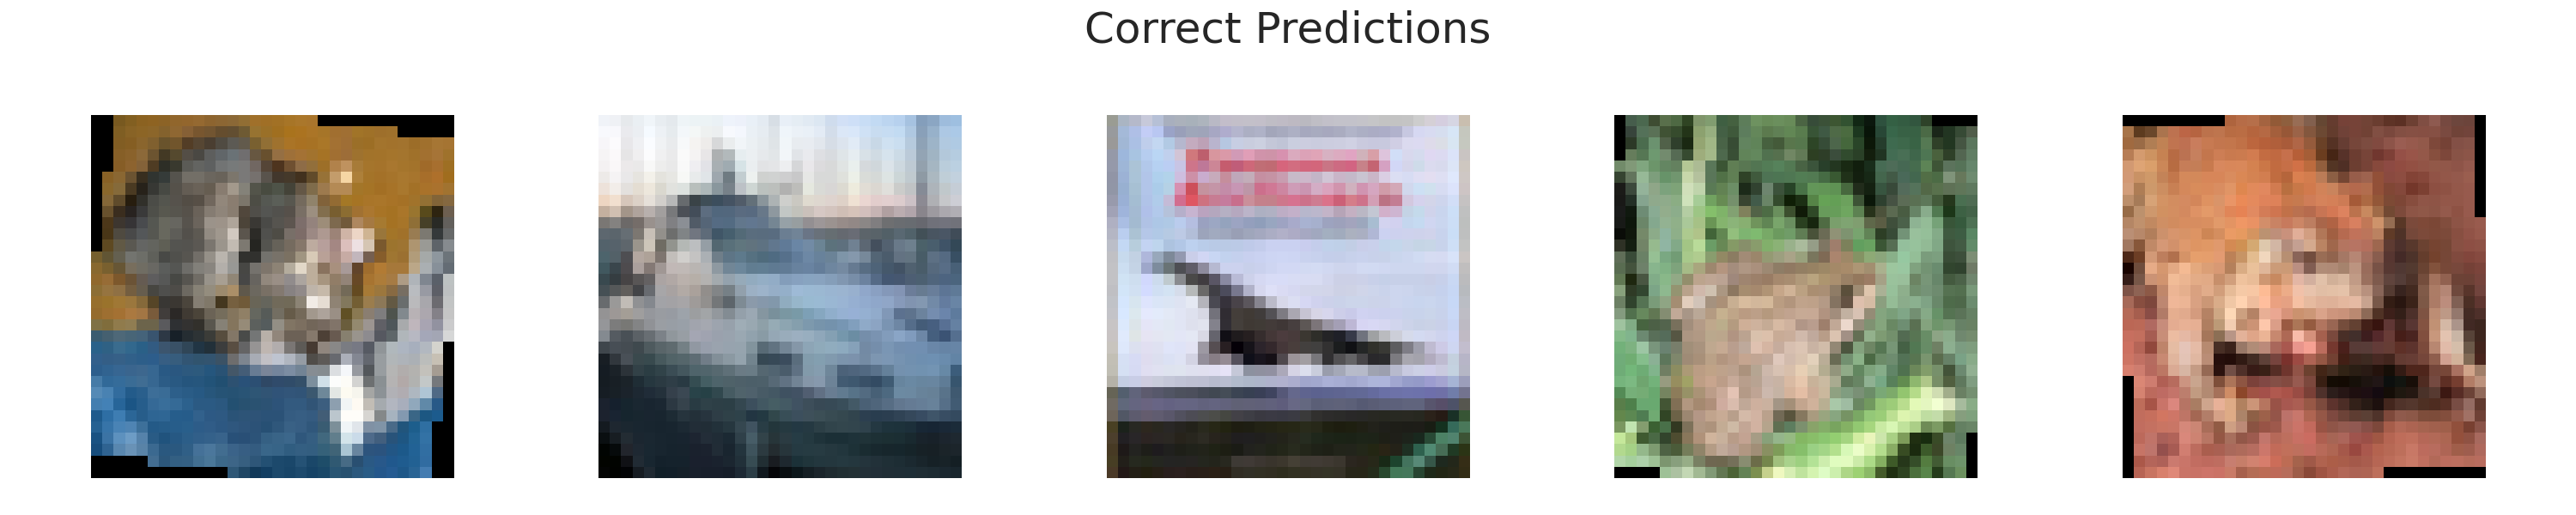
\includegraphics[width=\columnwidth]{images/correct_predictions.png}}
			\caption{Correct Predictions}
			\label{fig:correct_predictions}
		\end{figure}
		
		\item \textbf{Misclassified Images:}
		Conversely, this section highlights the images that were incorrectly classified by the model. Analyzing these images is crucial for identifying the limitations of the model and areas where it can be further trained for improved accuracy. The figure below displays a set of such misclassified images, each accompanied by the model's incorrect prediction. Reviewing these cases helps in understanding the model's weaknesses, particularly in scenarios where the visual features may be ambiguous or challenging to interpret.
		
		\begin{figure}[htbp]
			\centerline{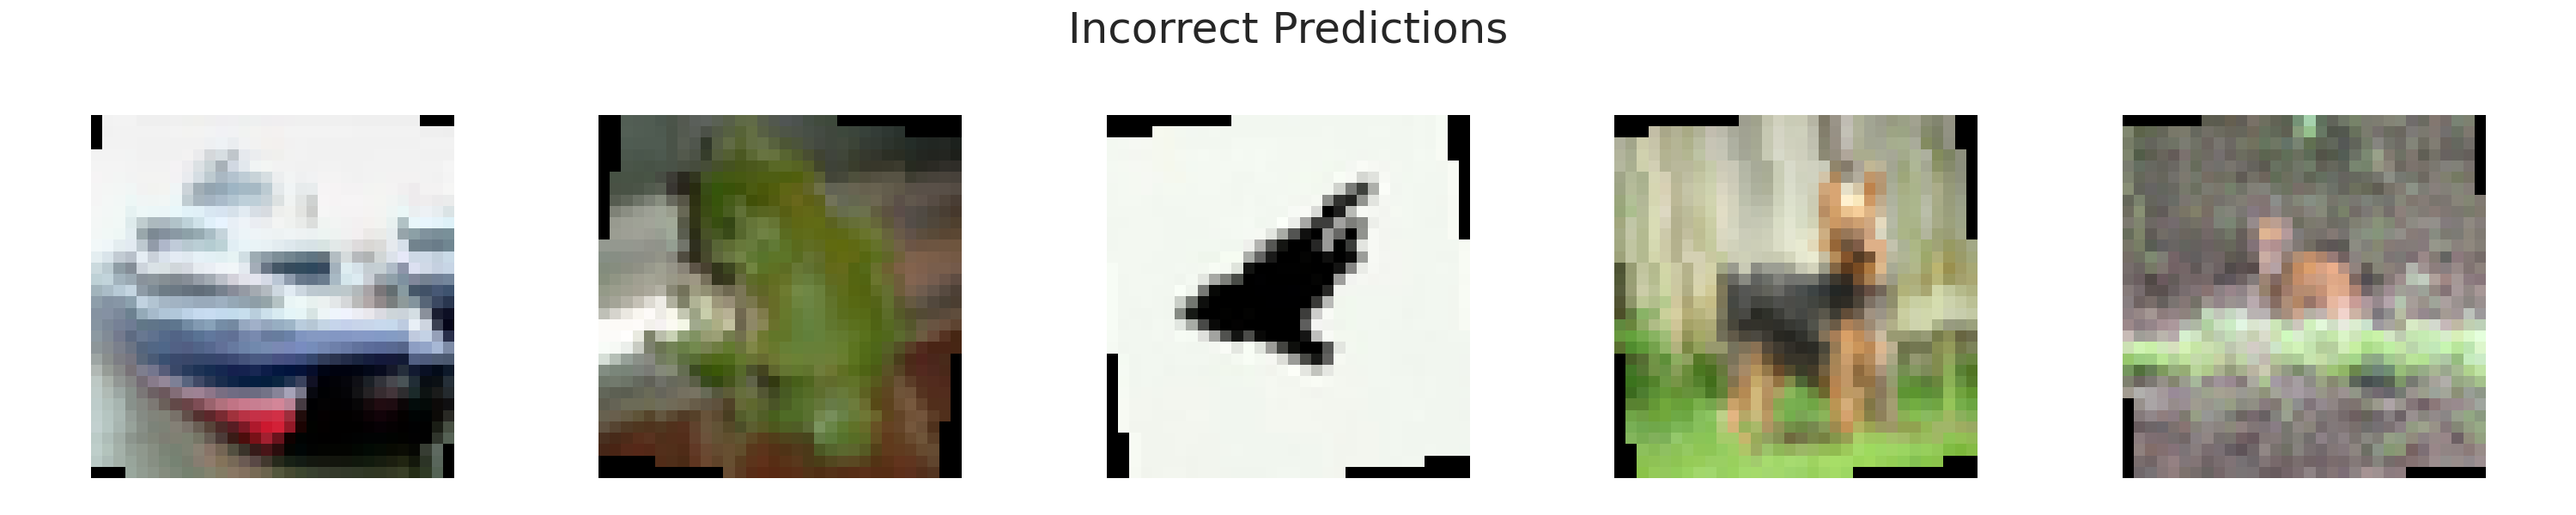
\includegraphics[width=\columnwidth]{images/incorrect_predictions.png}}
			\caption{Incorrect Predictions}
			\label{fig:incorrect_predictions}
		\end{figure}
	\end{enumerate}
	
	
	\section{Part3}
	In this section, I will discuss my approach to improving the classification performance and reducing the model size of a CNN for the CIFAR-10 dataset. The process is divided into three steps: analyzing the problem, modifying the model structure, and adjusting the training system.
	
	\subsection{Step 1: Problem Analysis}
	\begin{enumerate}
		\item \textbf{Existing Model Architecture and Parameters: }\\
		Based on the definitions of \texttt{Net()} in the original code, the layer details of the OriginNet Neural Network can be summarized in Table \ref{tab:origin_network_layers}. Additionally, the parameters and memory usage of the network are illustrated in Table \ref{tab:models_size}.
		
		\begin{table}[h]
			\centering
			\begin{tabular}{|l|l|r|}
				\hline
				\textbf{Layer Type} & \textbf{Output Shape} & \textbf{Param Count} \\ \hline
				Conv2d              & [1, 6, 33, 33]        & 78                   \\ \hline
				MaxPool2d           & [1, 6, 16, 16]        & 0                    \\ \hline
				Conv2d              & [1, 16, 17, 17]       & 400                  \\ \hline
				MaxPool2d           & [1, 16, 8, 8]         & 0                    \\ \hline
				Conv2d              & [1, 32, 7, 7]         & 2080                 \\ \hline
				MaxPool2d           & [1, 32, 3, 3]         & 0                    \\ \hline
				Linear              & [1, 120]              & 34680                \\ \hline
				Linear              & [1, 84]               & 10164                \\ \hline
				Linear              & [1, 10]               & 850                  \\ \hline
			\end{tabular}
			\caption{Layer Details of the OriginNet Neural Network}
			\label{tab:origin_network_layers}
		\end{table}        
		
		\item \textbf{Comparative Analysis of Lightweight Models: }\\
		Initially, I attempted to identify relatively lightweight models within the field of computer vision for static image analysis, which are known for their high recognition rates but with fewer parameters. Some examples of such architectures include ResNet18, DenseNet, VGG, InceptionV3, GoogLeNet, as well as mobile-oriented networks like MobileNet and EfficientNet. However, a comparison of their parameters revealed that these models have significantly larger sizes than the model used in this case, as shown in Table \ref{tab:models_size}. Therefore, I decided to focus on modifying the existing model to achieve the dual objectives of improving classification performance and reducing model size.
		
		\begin{table}[h]
			\centering
			\begin{tabular}{|c|c|c|}
				\hline
				\textbf{Model} & \textbf{Parameters} & \textbf{Memories} \\ \hline
				OriginNet      & 48252                & 0.19765 MB        \\ \hline
				ResNet18 \cite{b1}       & 11689512           & 46.839572 MB     \\ \hline
				DenseNet121 \cite{b2}    & 7978856            & 95.75856 MB      \\ \hline
				VGG16 \cite{b3}          & 138357544          & 1660.302816 MB   \\ \hline
				InceptionV3 \cite{b4}    & 27161264           & 325.947456 MB    \\ \hline
				GoogLeNet \cite{b5}      & 6624904            & 79.511136 MB     \\ \hline
				MobileNetV2 \cite{b6}    & 2236682            & 26.852472 MB     \\ \hline
			\end{tabular}
			\caption{Comparison of Existing Models Size}
			\label{tab:models_size}
		\end{table}
		
	\end{enumerate}

	\subsection{Step 2: Modifying the Model Structure}
	To achieve the objectives, there are some modifications:
	\begin{enumerate}
		\item \textbf{Adjustments to Convolutional Layers:}
		The number of filters in the convolutional layers was adjusted. Specifically, the filter count of the first convolutional layer was increased from 6 to 10 to capture more features at the initial stage. Concurrently, the filter counts in the second and third convolutional layers were reduced (from 16 to 12 in the second layer, and from 32 to 24 in the third layer) to decrease the number of parameters while still maintaining adequate feature extraction capabilities.
		
		\item \textbf{Depthwise Separable Convolution:}
		In the revised model, standard convolutions (nn.Conv2d) are replaced with depthwise separable convolutions. Depthwise separable convolutions, however, break this process into two distinct layers: depthwise convolutions that apply a single filter per input channel, and pointwise convolutions that combine the outputs of the depthwise layer. Mathematically, this can be represented as:
		
		\begin{equation}
			Y_{k} = \sum_{i=1}^{M} X_i * K_{i,k}
		\end{equation}
		
		Here, \(X_i\) is the input channel \(i\), \(K_{i,k}\) is the kernel for input channel \(i\) and output channel \(k\), and \(Y_{k}\) is the output channel \(k\). This approach significantly reduces the number of parameters and computational cost, while preserving the model's ability to learn rich, complex features.
		
		\item \textbf{Adjustments to Fully Connected Layers:}
		The model's fully connected layers have been optimized for efficiency. Specifically, the number of neurons in these layers was reduced; the first layer was decreased from 120 to 100 neurons, and the second from 84 to 64 neurons. This reduction is based on the principle that fewer neurons can still capture the essential features necessary for accurate classification, while simultaneously reducing the model's parameter count and computational load. The formula for calculating the parameters in a fully connected layer is:
		
		\begin{equation}
			P = (N_{in} + 1) \times N_{out}
		\end{equation}
		
		Where \(P\) is the number of parameters, \(N_{in}\) is the number of input neurons, \(N_{out}\) is the number of output neurons, and the "+1" accounts for the bias term.
		
		\item \textbf{Incorporation of Batch Normalization:}
		Batch normalization was introduced after each convolutional and fully connected layer. This technique normalizes the input layer by adjusting and scaling the activations. The formula for batch normalization is given by:
		
		\begin{equation}
			BN(x) = \gamma \left( \frac{x - \mu}{\sqrt{\sigma^2 + \epsilon}} \right) + \beta
		\end{equation}
		
		Where \(x\) is the input, \(\mu\) and \(\sigma^2\) are the mean and variance computed over the batch, \(\epsilon\) is a small number to avoid division by zero, and \(\gamma\) and \(\beta\) are learnable parameters for scale and shift. Batch normalization helps in reducing internal covariate shift, speeding up training, and improving the overall performance of the model.
		
		\item \textbf{Introduction of Dropout Layers:}
		Dropout layers were strategically placed between the fully connected layers. During training, dropout randomly sets a fraction of input units to zero at each update, which helps in preventing overfitting. The dropout rate typically ranges from 0.2 to 0.5; a higher rate implies more units are dropped. The mathematical representation of dropout is:
		
		\begin{equation}
			Y = X \odot M
		\end{equation}
		
		Where \(X\) is the input, \(M\) is a binary mask where entries are drawn from a Bernoulli distribution with probability equal to the dropout rate, and \(\odot\) represents element-wise multiplication. Dropout effectively creates a thinned version of the network, leading to better generalization on unseen data.
		
		\item \textbf{Modified Model Architecture:}
		Layer Details of the ModifiedNet Neural Network is in Table \ref{tab:modified_network_layers}, the Model Size of ModifiedNet in Table \ref{tab:mode_size_modified_net}, and the ModifiedNet Neural Network Model Architecture in Figure \ref{fig:modified_net_arch}.
		
		\begin{table}[h]
			\centering
			\begin{tabular}{|c|c|c|}
				\hline
				\textbf{Model} & \textbf{Parameters} & \textbf{Memories} \\ \hline
				ModifiedNet      &         35730            &       0.001194 MB            \\ \hline
			\end{tabular}
			\caption{Model Size of ModifiedNet}
			\label{tab:mode_size_modified_net}
		\end{table}
		
		\begin{table}[h]
			\centering
			\begin{tabular}{|l|l|r|}
				\hline
				\textbf{Layer Type} & \textbf{Output Shape} & \textbf{Param Count} \\ \hline
				Conv2d              & [1, 8, 32, 32]       & 224                  \\ \hline
				BatchNorm2d         & [1, 8, 32, 32]       & 16                   \\ \hline
				MaxPool2d           & [1, 8, 16, 16]       & 0                    \\ \hline
				Conv2d              & [1, 12, 16, 16]      & 876                  \\ \hline
				BatchNorm2d         & [1, 12, 16, 16]      & 24                   \\ \hline
				MaxPool2d           & [1, 12, 8, 8]        & 0                    \\ \hline
				Conv2d              & [1, 16, 8, 8]        & 1744                 \\ \hline
				BatchNorm2d         & [1, 16, 8, 8]        & 32                   \\ \hline
				MaxPool2d           & [1, 16, 4, 4]        & 0                    \\ \hline
				Linear              & [1, 100]             & 25700                \\ \hline
				Dropout             & [1, 100]             & 0                    \\ \hline
				Linear              & [1, 64]              & 6464                 \\ \hline
				Dropout             & [1, 64]              & 0                    \\ \hline
				Linear              & [1, 10]              & 650                  \\ \hline
			\end{tabular}
			\caption{Layer Details of the ModifiedNet Neural Network}
			\label{tab:modified_network_layers}
		\end{table}
		
		\item \textbf{Performance of the Modified Model:}
		    The modifications implemented in the architecture of the model have led to substantial improvements in its performance metrics. The table below illustrates a comparative analysis between the original OriginNet model and the ModifiedNet. The precision value increased from 0.5525 to 0.6524, and the recall value saw a similar improvement. Consequently, the F1 score, which is a harmonic mean of precision and recall, also improved, indicating a more balanced performance between the precision and recall of the model.
		
		\begin{table}[h]
			\centering
			\begin{tabular}{|c|c|c|c|}
				\hline
				\textbf{Model} & \textbf{Precision Value} & \textbf{Recall Value} & \textbf{F1 Score} \\ \hline
				OriginNet      & 0.5525                   & 0.5573                & 0.5521            \\ \hline
				ModifiedNet    & 0.6524                   & 0.6576                & 0.6536            \\ \hline
			\end{tabular}
			\caption{}
			\label{tab:my-table}
		\end{table}
		
%		\begin{figure}[htbp]
%			\centerline{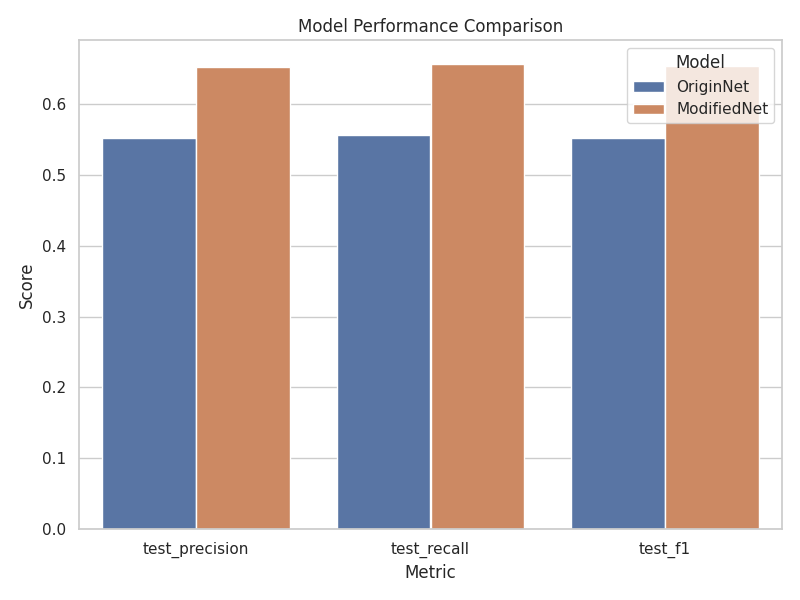
\includegraphics[width=\columnwidth]{images/model_arch_performance_comparison.png}}
%			\caption{Comparison of OriginNet and ModifiedNet}
%			\label{fig:model_arch_performance_comparison}
%		\end{figure}
		
	\begin{figure}[htbp]
		\centerline{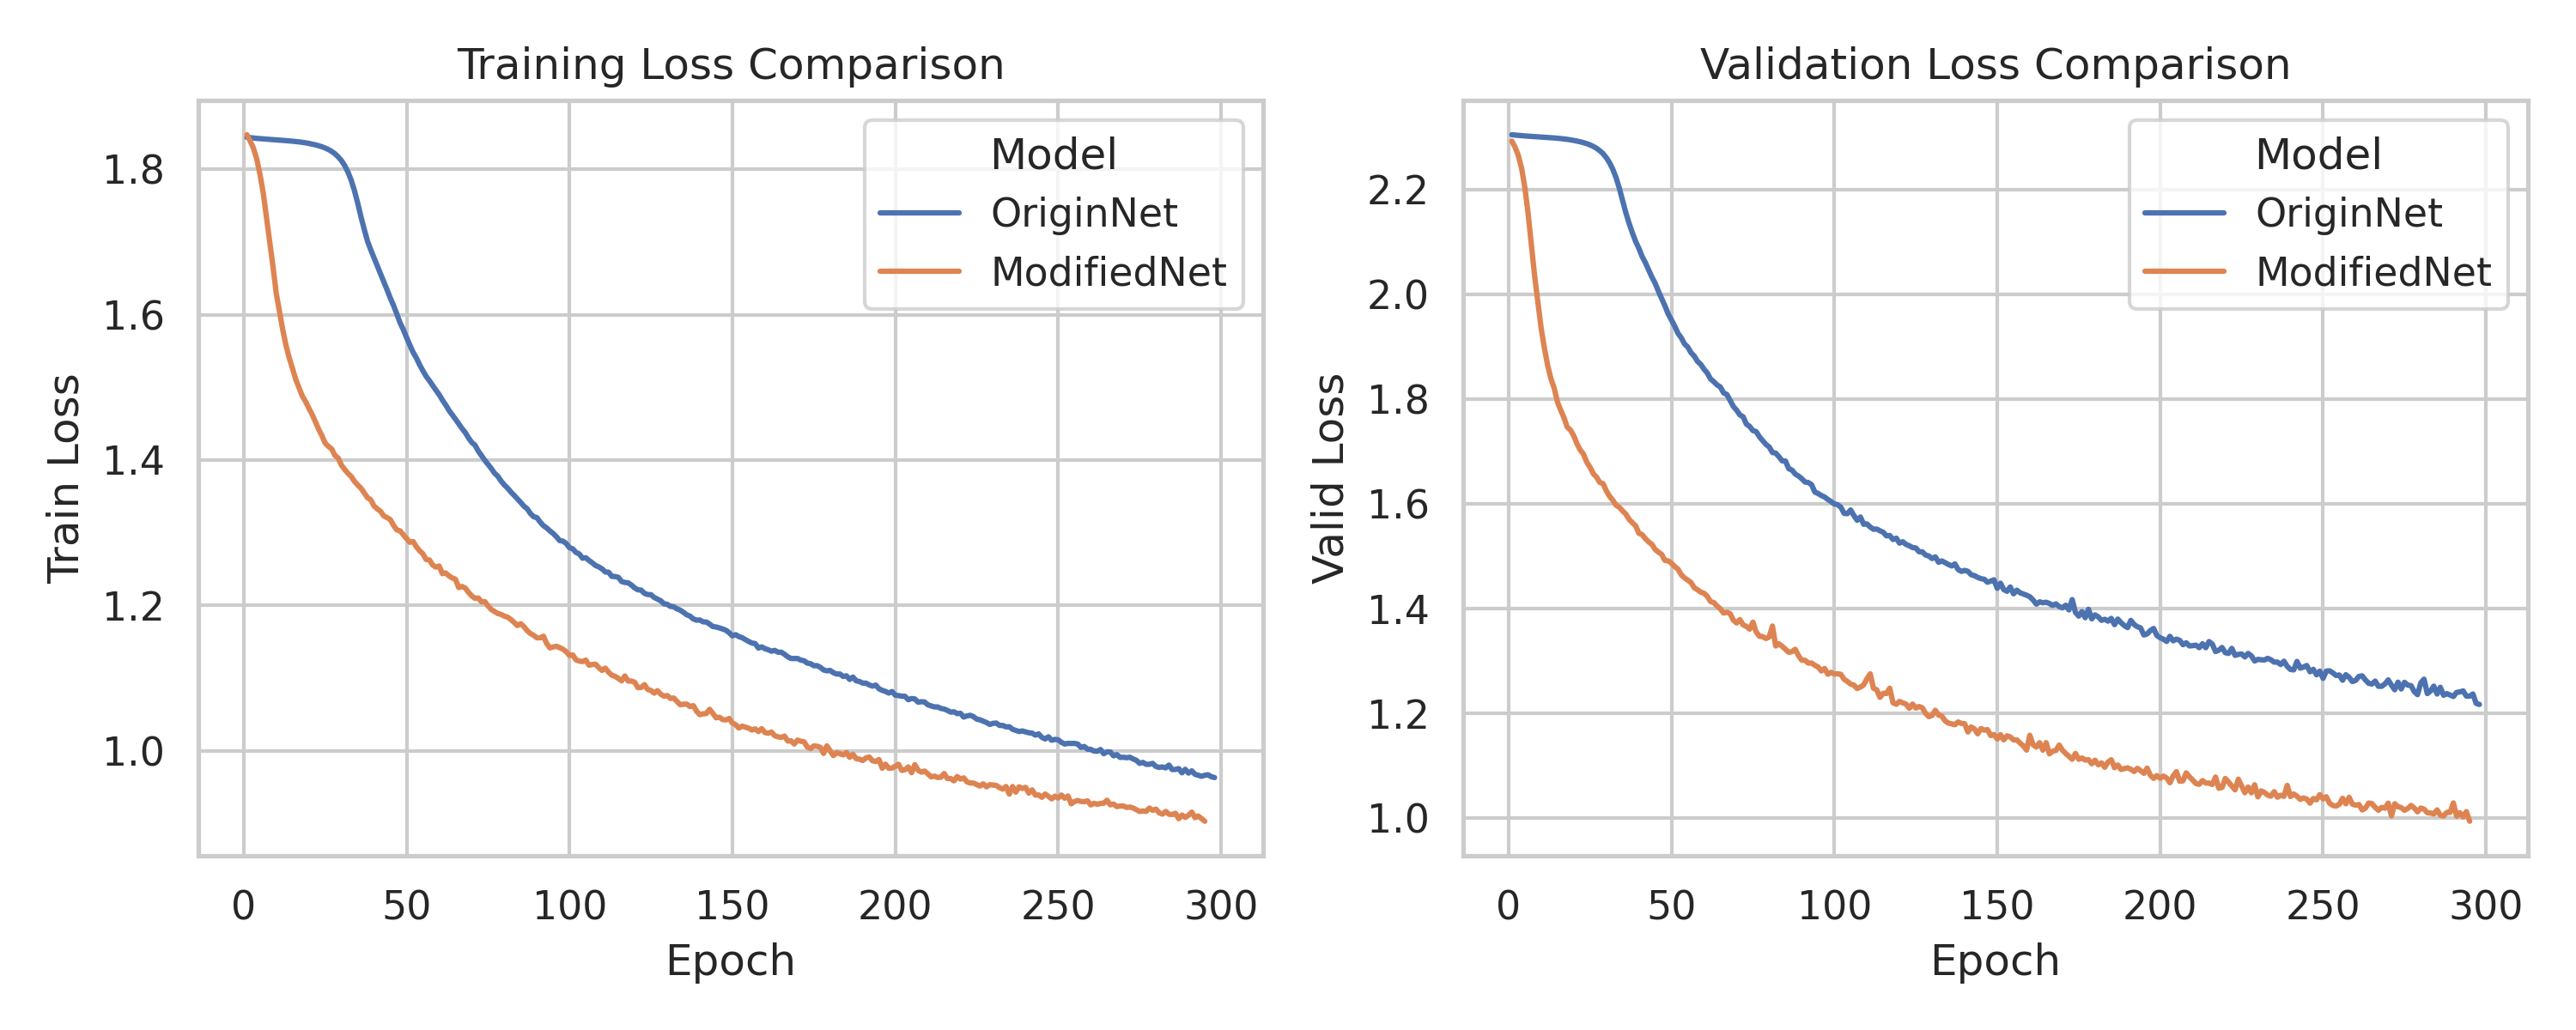
\includegraphics[width=\columnwidth]{images/loss_comparison.png}}
		\caption{Loss Comparison between OriginNet and ModifiedNet}
		\label{fig:loss_comparison}
	\end{figure}
	
	\begin{figure}[htbp]
		\centerline{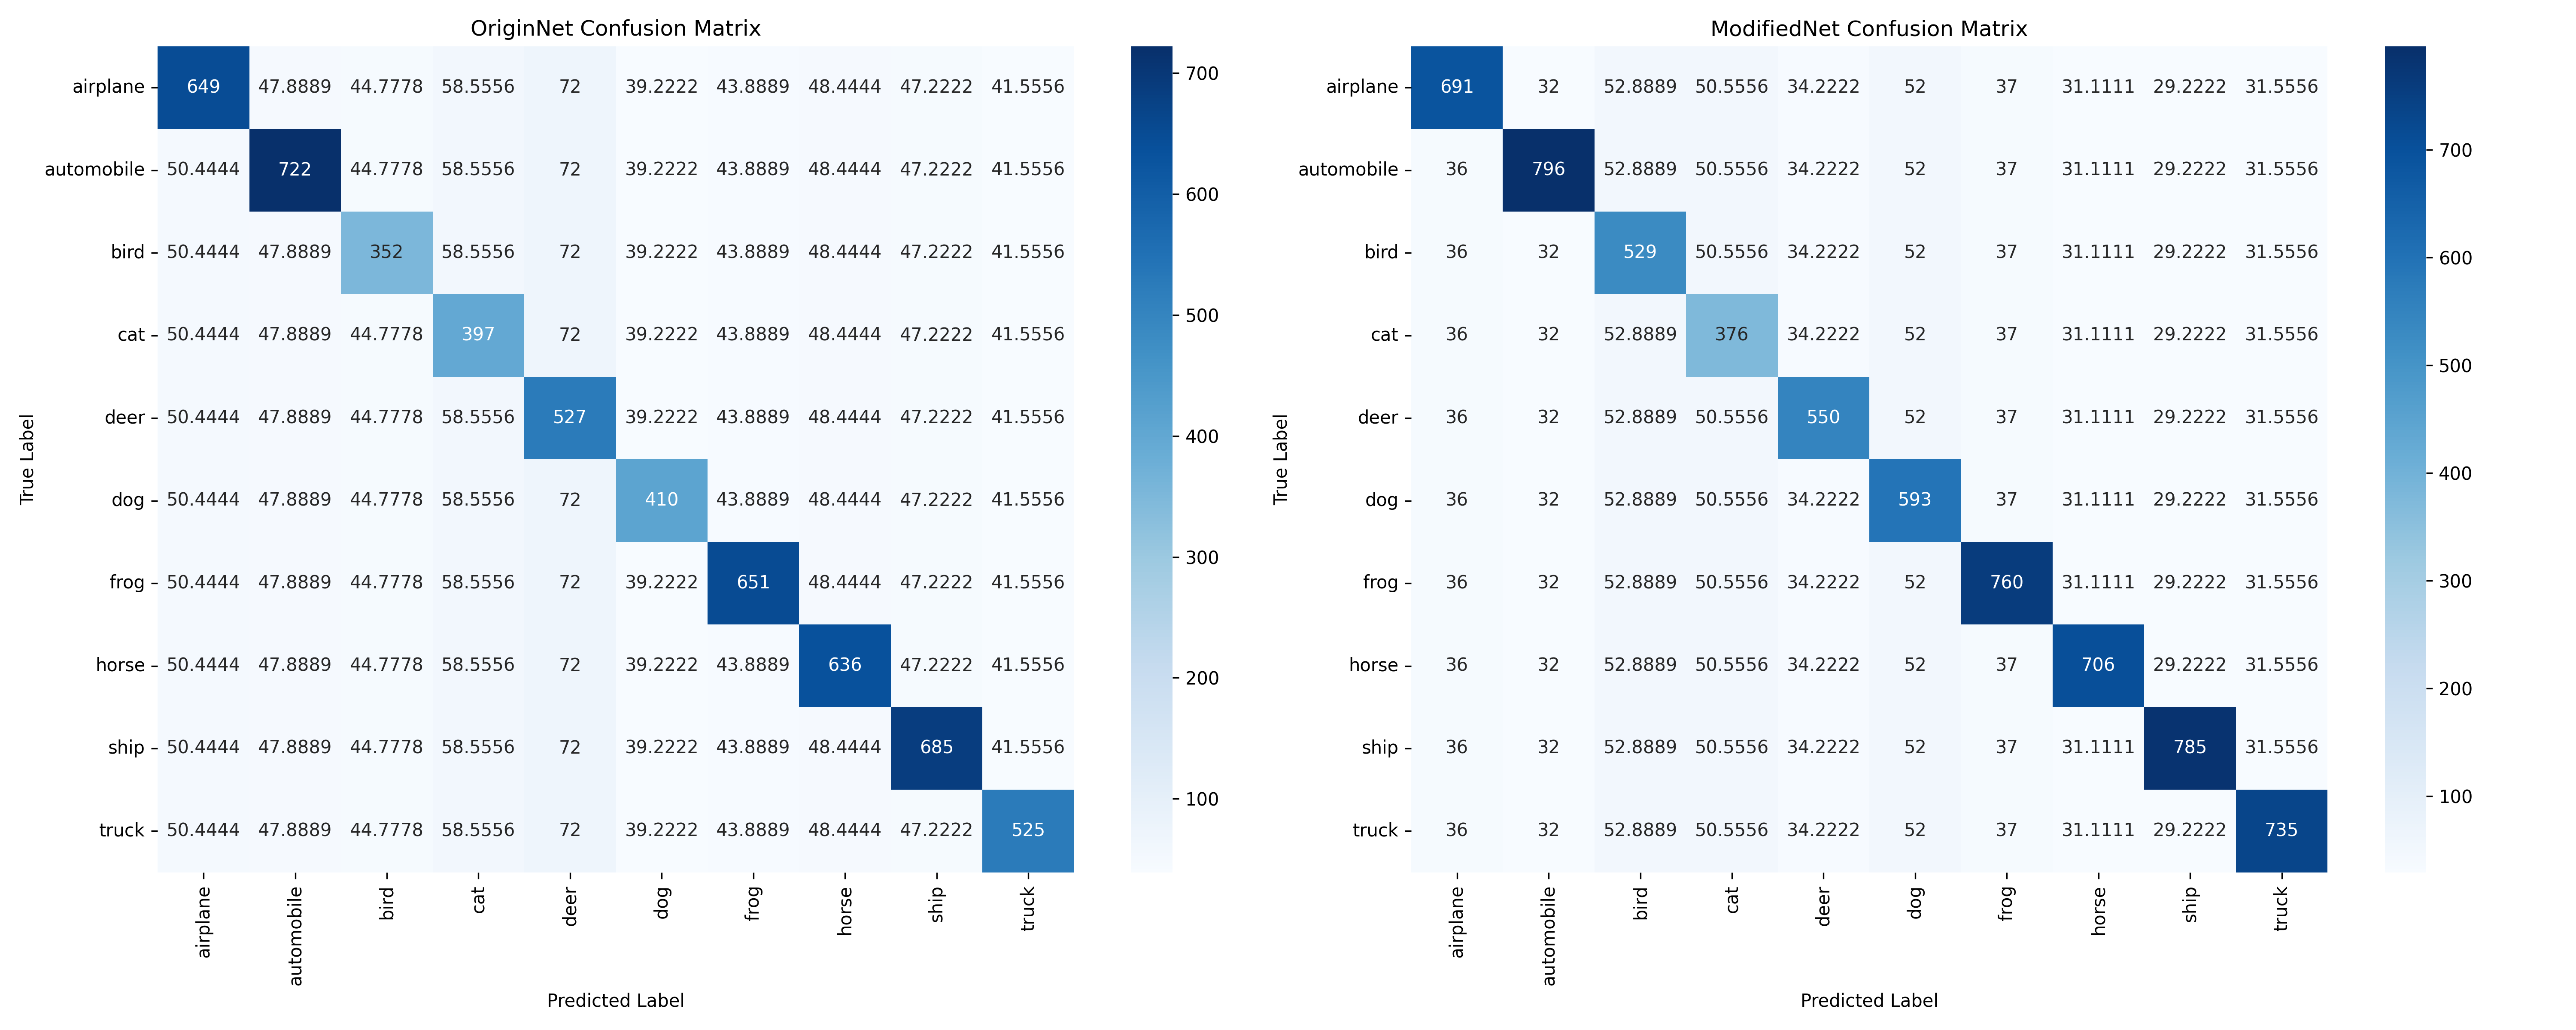
\includegraphics[width=\columnwidth]{images/confusion_matrices_comparison.png}}
		\caption{Confusion Matrices Comparison}
		\label{fig:confusion_matrices_comparison}
	\end{figure}
	\end{enumerate}
	
	\begin{figure*}
		\centering
		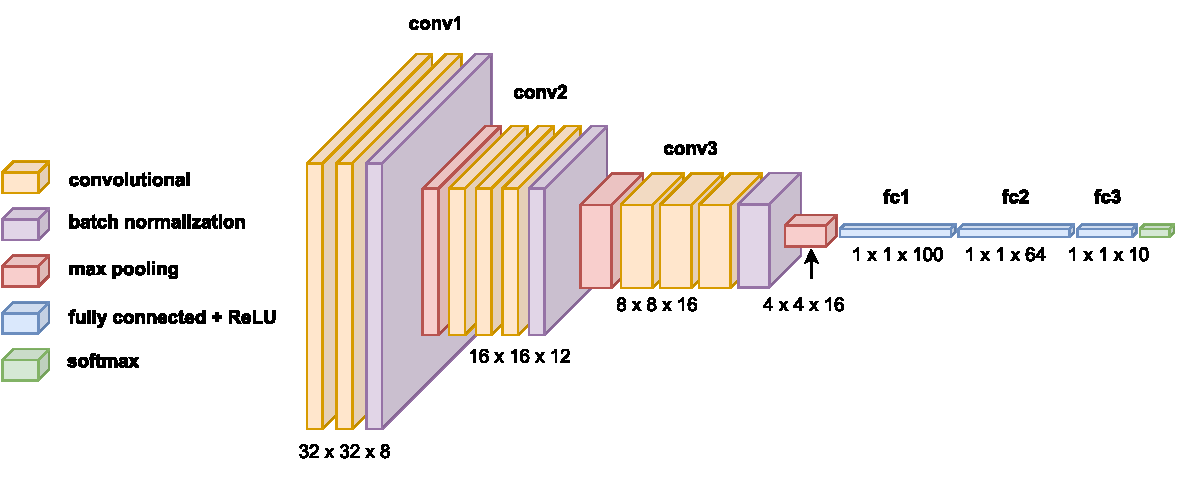
\includegraphics[width=6.2in]{drawio/modifiedNet.pdf}
		\caption{ModifiedNet Neural Network Model Architecture}
		\label{fig:modified_net_arch}
	\end{figure*}
	
	\subsection{Step 3: Adjusting the Training System}
	An ablation study method was adopted to investigate the factors influencing the model's classification performance. An ablation study systematically modifies or removes certain components of a model to understand their impact on the model's performance, helping to identify crucial elements for effectiveness and efficiency.
	
	\begin{enumerate}
		\item \textbf{Learning Rate Adjustment:}
		Different learning rates were experimented with, including 0.0001, 0.0005, 0.001, 0.005, and 0.01. The optimal performance under the ModifiedNet model's architecture was observed at a learning rate of 0.005. This rate offers the best balance between convergence speed and accuracy for ModifiedNet, as illustrated in the figure and table below.
		
		\begin{figure}[htbp]
			\centerline{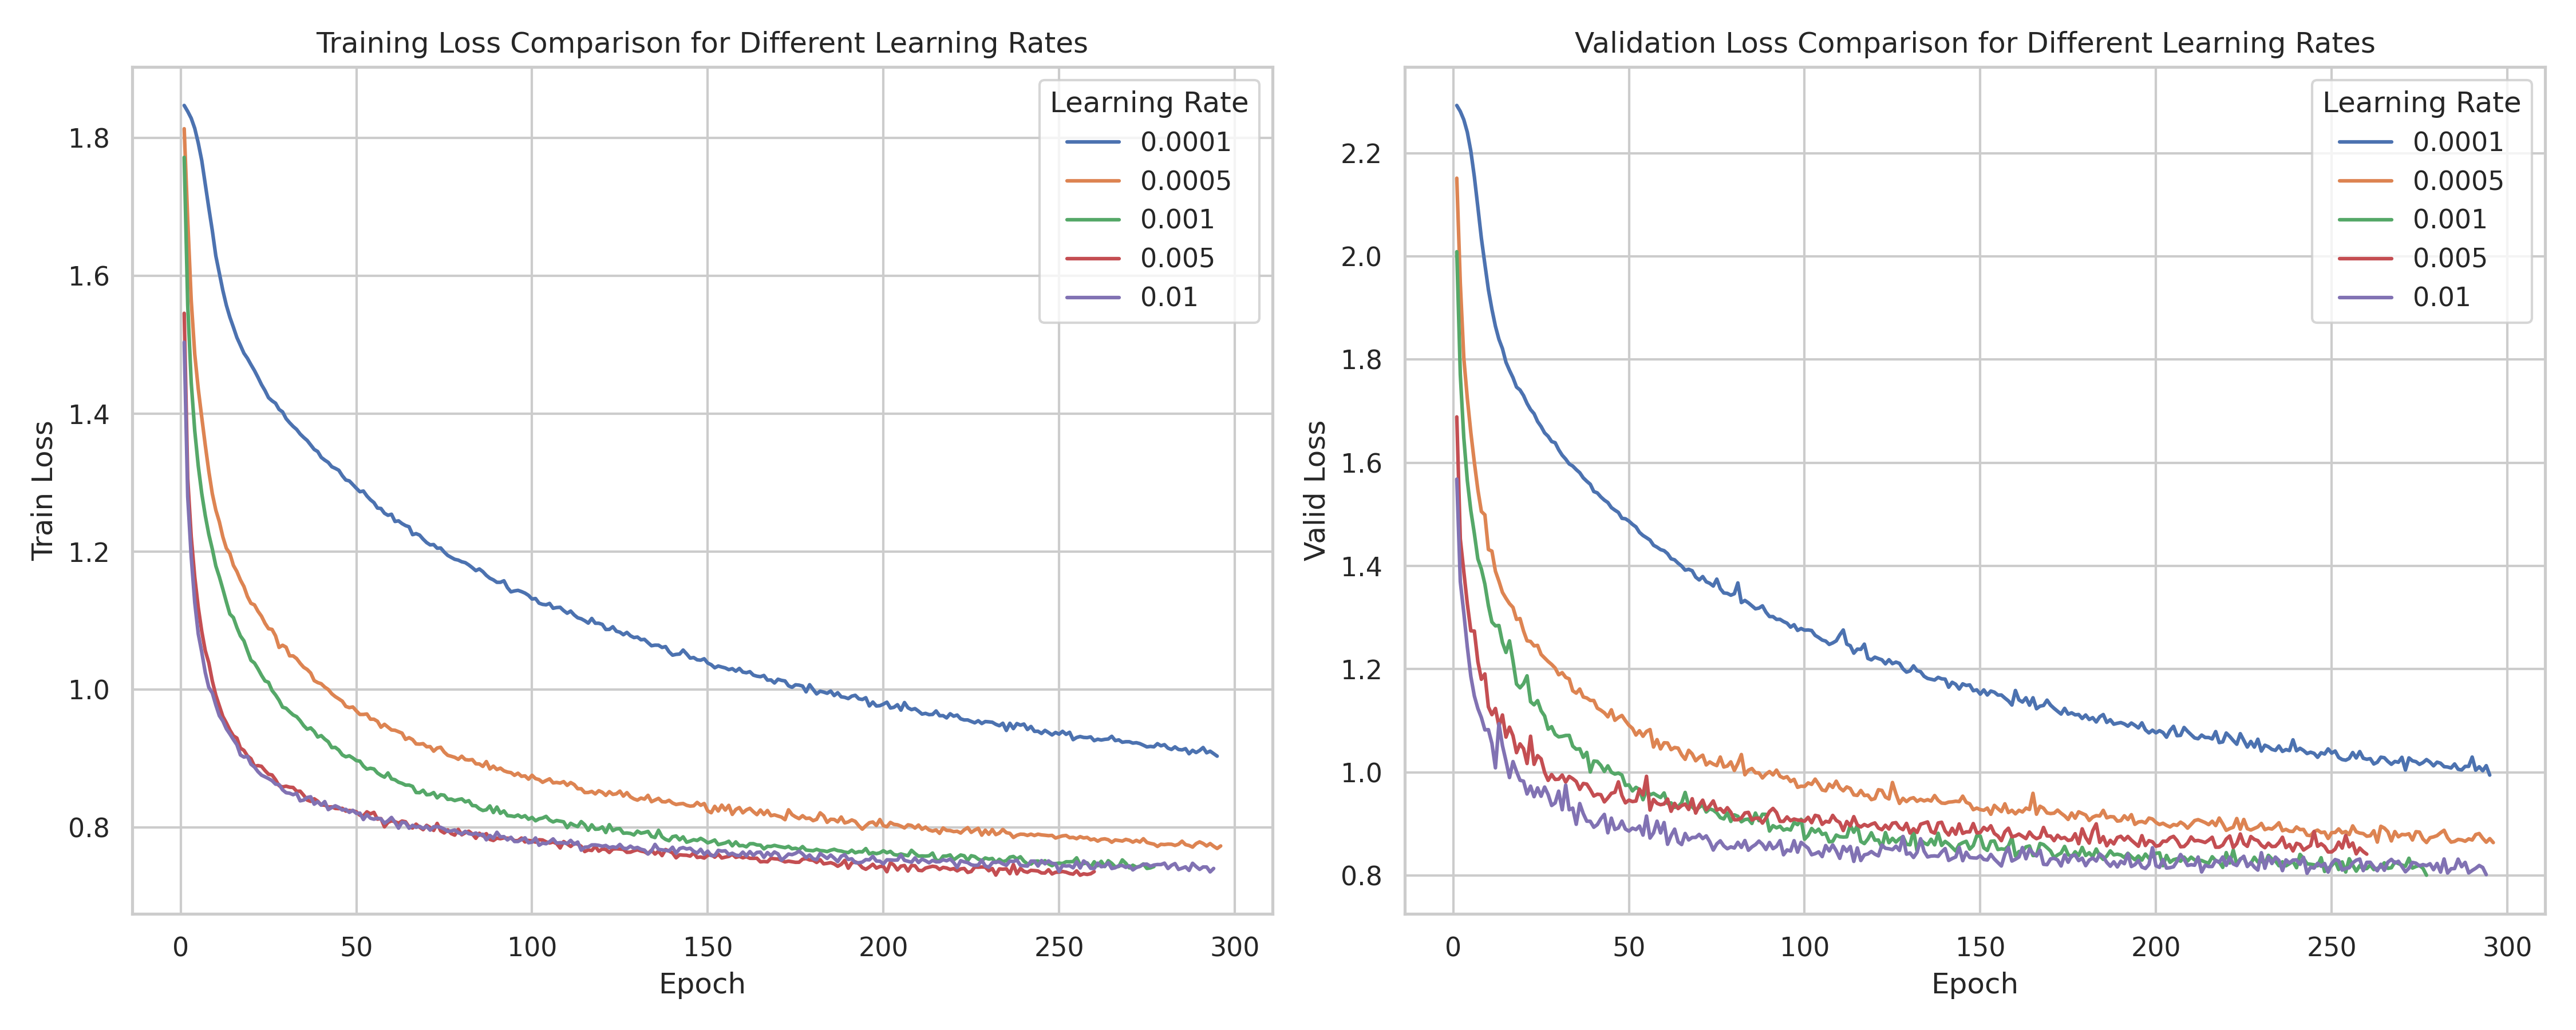
\includegraphics[width=\columnwidth]{images/loss_comparison_lr.png}}
			\caption{Loss Comparison by Learning Rate}
			\label{fig:loss_comparison_lr}
		\end{figure}
		
		\begin{table}[h]
			\centering
			\begin{tabular}{|c|c|c|c|c|}
				\hline
				\textbf{Model} & \textbf{Accuracy} & \textbf{Parameters} & \textbf{Memories} & \textbf{Train Time} \\ \hline
				baseline       & 71.2\%  & 35730 & 0.153282 MB & 33min \\ \hline
				+lr=0.0001     & 65.21\% & 35730 & 0.153282 MB & 28min \\ \hline
				+lr=0.0005     & 69.62\% & 35730 & 0.153282 MB & 31min \\ \hline
				+lr=0.005      & 72.8\%  & 35730 & 0.153282 MB & 29min \\ \hline
				+lr=0.01       & 71.49\% & 35730 & 0.153282 MB & 31min \\ \hline
			\end{tabular}
			\caption{Ablation Study on Learning Rate Adjustments}
			\label{tab:lr_adjustments}
		\end{table}
	
		\item \textbf{Optimizer Comparison:}
		In the pursuit of optimizing model performance, we compared four different optimizers: SGD (Stochastic Gradient Descent), Adam, RMSprop, and Adagrad. Each of these optimizers has distinct mechanisms and principles:
		
		\textbf{SGD:} The Stochastic Gradient Descent optimizer is a simple yet effective approach. It updates model parameters \(\theta\) using the formula: 
		\begin{equation}
			\theta = \theta - \eta \cdot \nabla_\theta J( \theta; x^{(i)}; y^{(i)})
		\end{equation}
		where \(\eta\) is the learning rate, and \(\nabla_\theta J\) is the gradient of the cost function \(J\) with respect to the parameters \(\theta\), evaluated at a randomly chosen data point \((x^{(i)}, y^{(i)})\).
		
		\textbf{Adam:} Adam (Adaptive Moment Estimation) combines the benefits of two other extensions of stochastic gradient descent: AdaGrad and RMSProp. It calculates adaptive learning rates for each parameter through moment estimates:
		\begin{equation}
			\theta = \theta - \frac{\eta}{\sqrt{\hat{v}} + \epsilon} \hat{m}
		\end{equation}
		where \(\hat{m}\) and \(\hat{v}\) are estimates of the first and second moments of the gradients.
		
		\textbf{RMSprop:} RMSprop addresses the diminishing learning rates problem of AdaGrad. It uses a moving average of squared gradients to normalize the gradient:
		\begin{equation}
			\theta = \theta - \frac{\eta}{\sqrt{E[g^2] + \epsilon}} g
		\end{equation}
		where \(E[g^2]\) is the moving average of the squared gradients.
		
		\textbf{Adagrad:} Adagrad adapts the learning rate to the parameters, performing smaller updates for parameters associated with frequently occurring features:
		\begin{equation}
			\theta = \theta - \frac{\eta}{\sqrt{G_{ii} + \epsilon}} g_i
		\end{equation}
		where \(G_{ii}\) is a diagonal matrix where each diagonal element \(i, i\) is the sum of the squares of the gradients w.r.t. \(\theta_i\) up to time step \(t\).
		
		After extensive testing and comparison, as illustrated in the figure and table below, it was found that the SGD optimizer delivered the best performance in terms of accuracy and training time for the ModifiedNet model. This underscores the efficacy of SGD in certain contexts, despite the more complex mechanisms of other optimizers.
		
		\begin{figure}[htbp]
			\centerline{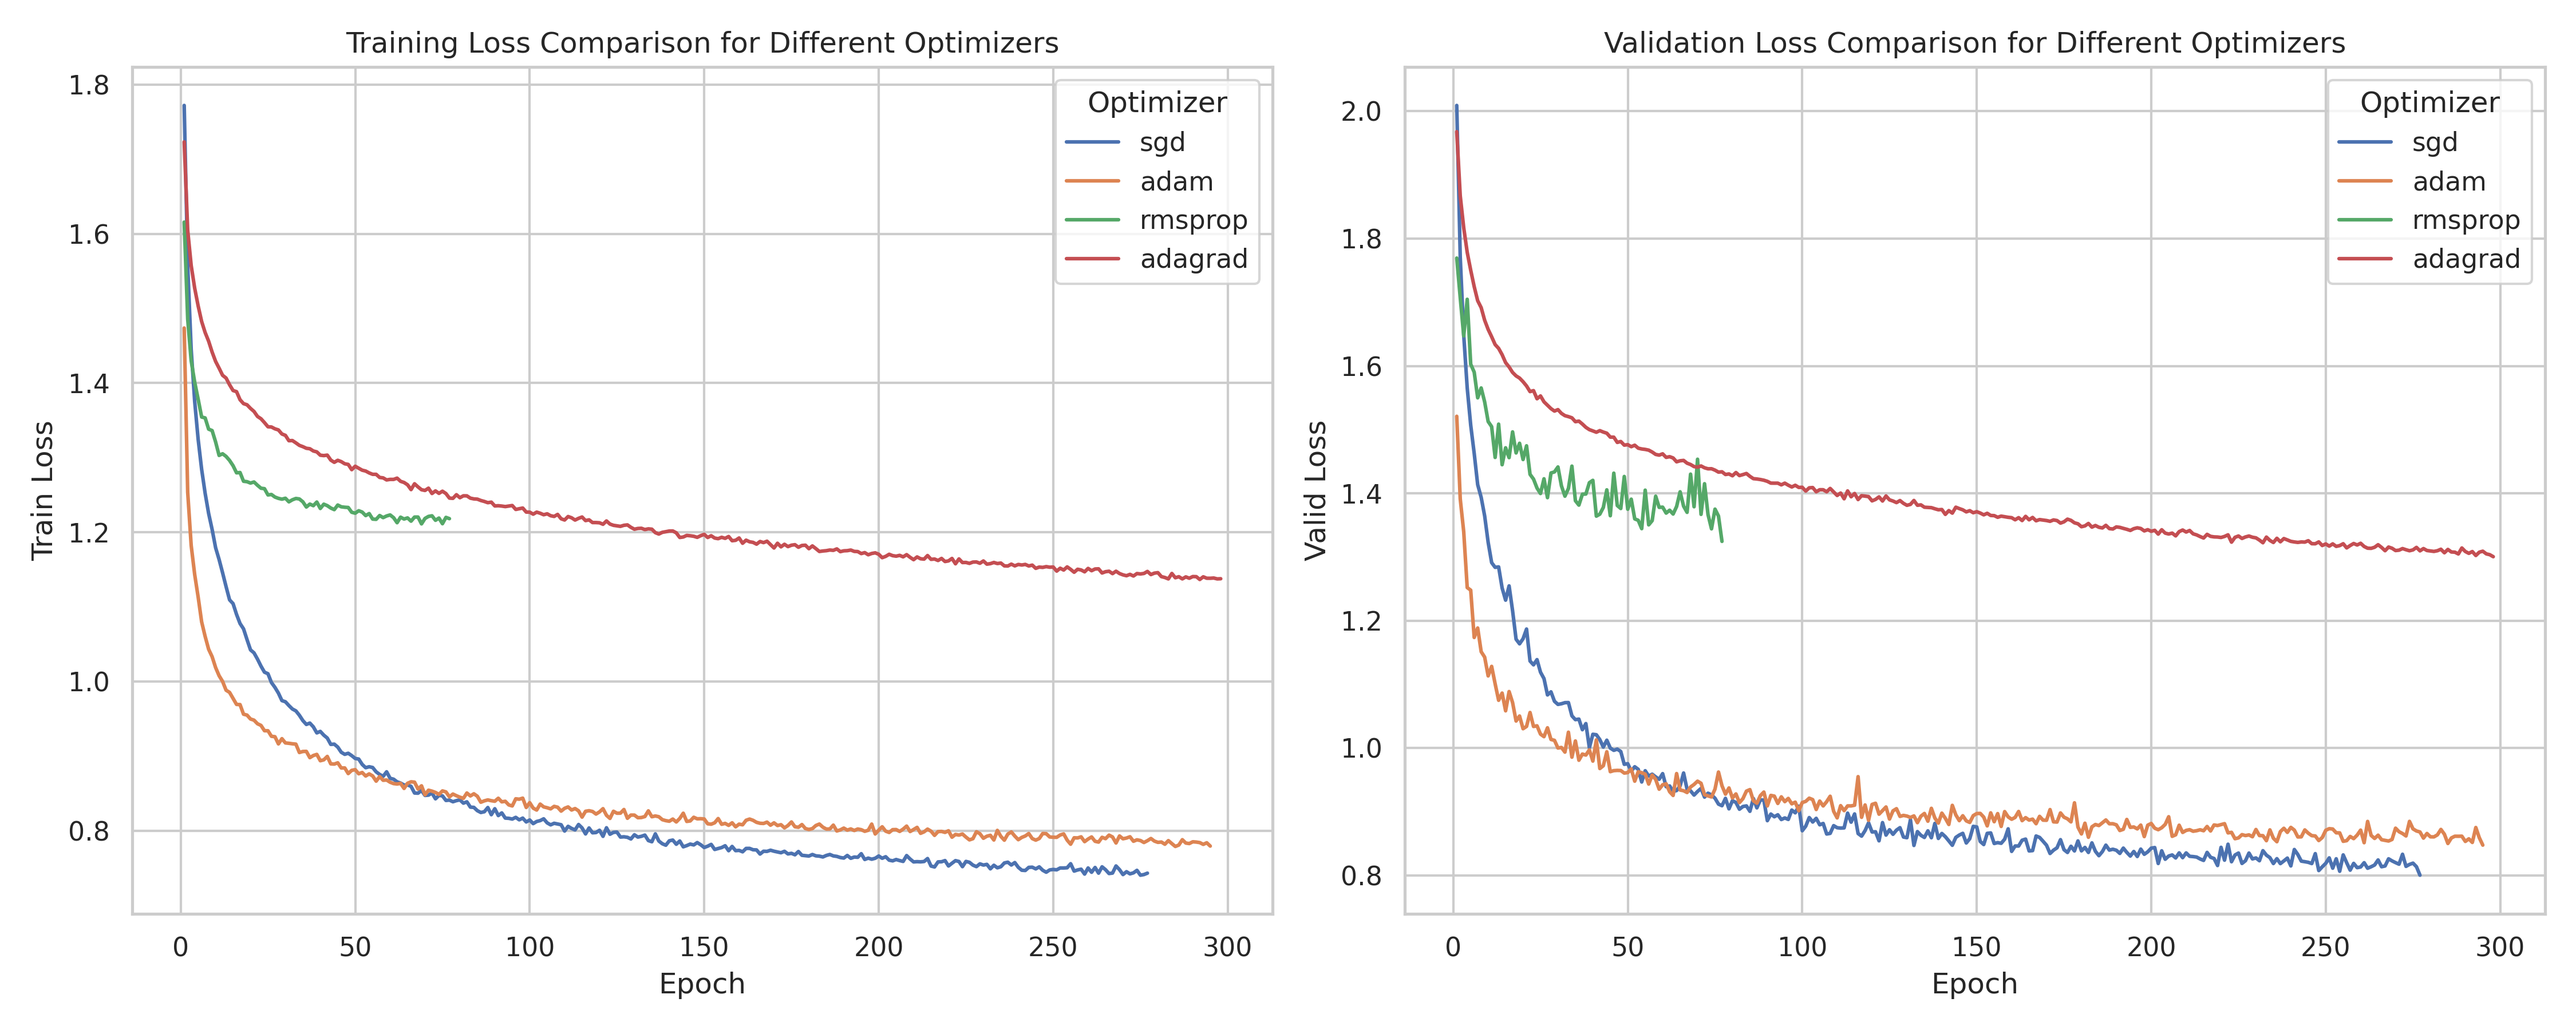
\includegraphics[width=\columnwidth]{images/loss_comparison_optimizer.png}}
			\caption{Loss Comparison by Optimizer}
			\label{fig:loss_comparison_op}
		\end{figure}
		
		\begin{table}[h]
			\centering
			\begin{tabular}{|c|c|c|c|c|}
				\hline
				\textbf{Model} & \textbf{Accuracy} & \textbf{Parameters} & \textbf{Memories} & \textbf{Train Time} \\ \hline
				baseline       & 72.8\%  & 35730 & 0.153282 MB & 29min\\ \hline
				+op=adam       & 70.43\% & 35730 & 0.153282 MB & 31min \\ \hline
				+op=rmsprop    & 48.64\% & 35730 & 0.153282 MB & 33min \\ \hline
				+op=adagrad    & 53.48\% & 35730 & 0.153282 MB & 34min \\ \hline
			\end{tabular}
			\caption{Optimizer Comparison Results}
			\label{tab:op_adjustments}
		\end{table}
		
		\item \textbf{Loss Function Comparison:}
		In the quest to refine the model's performance, we conducted a comparative analysis of different loss functions. Given that CIFAR-10 is a balanced dataset, a straightforward cross-entropy loss function typically outperforms a weighted cross-entropy approach. Cross-entropy loss, denoted as CE, is defined as:
		
		\begin{equation}
			CE = -\sum_{c=1}^{M} y_{o,c} \log(p_{o,c})
		\end{equation}
		
		where \(M\) is the number of classes, \(y\) is a binary indicator (0 or 1) if class label \(c\) is the correct classification for observation \(o\), and \(p\) is the predicted probability of observation \(o\) being of class \(c\).
		
		However, to further enhance the model's ability to generalize, we explored the use of label smoothing as an alternative. Label smoothing works by softening the hard targets (0s and 1s) in the training data, which can lead to a more robust model. The smoothed label for a class \(c\) is calculated as:
		
		\begin{equation}
			LS(y_{c}) = (1 - \alpha) \cdot y_{c} + \frac{\alpha}{M}
		\end{equation}
		
		where \(\alpha\) is the smoothing parameter and \(M\) is the number of classes. This approach can help in reducing overconfidence in predictions and provides a regularizing effect.
		
		Our experiments revealed that while cross-entropy loss is effective for balanced datasets like CIFAR-10, incorporating label smoothing provided a noticeable improvement in the model's ability to handle ambiguous or noisy labels. This was reflected in the enhanced performance metrics observed during validation.
		
	\end{enumerate}
	
	\section{Conclusion}
	This report has presented a comprehensive analysis and modification of a CNN framework for CIFAR-10 image classification. The study began with an in-depth examination of the convolutional kernel and the loss function, highlighting their pivotal roles in the CNN's ability to process and learn from CIFAR-10's small, colored images. Through mathematical formulations and detailed discussions, the intricacies of these components were elucidated, demonstrating their impact on the model's performance.
	
	In the subsequent sections, the report delved into the training, testing, and performance evaluation of the ModifiedNet model. A significant part of this process involved comparing various architectures and optimization strategies. The ablation study method was instrumental in isolating and understanding the effects of different learning rates, optimizers, and loss functions on the model's accuracy and efficiency.
	
	The ModifiedNet model, with its tailored convolutional layers, depthwise separable convolutions, optimized fully connected layers, batch normalization, and dropout layers, emerged as a significantly improved version of the original model. Not only did it demonstrate enhanced accuracy and efficiency, but it also maintained a balance between computational resource utilization and model complexity.
	
	In conclusion, this report successfully achieved its objectives of improving classification performance and reducing model size for CIFAR-10 image classification. The innovative approaches and modifications applied to the CNN framework have not only enhanced its performance but also provided a template for future research in image classification tasks. The insights gained from this study can be leveraged to further refine CNN models, paving the way for more efficient and accurate image classification systems.
	
	\begin{thebibliography}{00}
		\bibitem{b1} K. He, X. Zhang, S. Ren, and J. Sun, "Deep Residual Learning for Image Recognition," 2016 IEEE Conference on Computer Vision and Pattern Recognition (CVPR), 2016.
		\bibitem{b2} G. Huang, Z. Liu, L. Van Der Maaten, and K. Q. Weinberger, "Densely Connected Convolutional Networks," 2017 IEEE Conference on Computer Vision and Pattern Recognition (CVPR), 2017.
		\bibitem{b3} K. Simonyan and A. Zisserman, "Very Deep Convolutional Networks for Large-Scale Image Recognition," International Conference on Learning Representations, 2015.
		\bibitem{b4} C. Szegedy, V. Vanhoucke, S. Ioffe, J. Shlens, and Z. Wojna, "Rethinking the Inception Architecture for Computer Vision," 2016 IEEE Conference on Computer Vision and Pattern Recognition (CVPR), 2016.
		\bibitem{b5} C. Szegedy, W. Liu, Y. Jia, P. Sermanet, S. Reed, D. Anguelov, D. Erhan, V. Vanhoucke, and A. Rabinovich, "Going Deeper with Convolutions," 2015 IEEE Conference on Computer Vision and Pattern Recognition (CVPR), 2015.
		\bibitem{b6} M. Sandler, A. Howard, M. Zhu, A. Zhmoginov, and L. Chen, "MobileNetV2: Inverted Residuals and Linear Bottlenecks," 2018 IEEE/CVF Conference on Computer Vision and Pattern Recognition, 2018.
	\end{thebibliography}
	
	\appendix
	\section{Appendix}
	
	\subsection{Project File Structure}
	\begin{verbatim}
		.
		|-- ablation_study
		|   |-- baseline.py
		|   `-- ... ...
		|-- data
		|-- evaluate.py
		|-- images
		|-- jupyter
		|   |-- CIFARNotes.ipynb
		|   `-- CIFAROriginal.ipynb
		|-- logs
		|   |-- evaluate_2023-12-08_01-29-31.log
		|   `-- ... ...
		|-- main.py
		|-- models
		|   |-- modifiedNet.pt
		|   `-- ... ...
		|-- outputs
		|   |-- evaluate_2023-12-08_01-29-31.csv
		|   `-- ... ...
		|-- pytorch_cifar_classification
		|   |-- data
		|   |   `-- cifar-10-python.tar.gz
		|   |-- datasets
		|   |   |-- data_loader_manager.py
		|   |-- models
		|   |   |-- modified_net.py
		|   |   |-- origin_net.py
		|   |   `-- resnet18.py
		|   `-- utils
		|       |-- logger.py
		|       |-- metrics.py
		|       |-- model_utils.py
		|       |-- options.py
		|       |-- plotting_utils.py
		|       |-- predictor.py
		|       |-- recorder.py
		|       |-- saver.py
		|       `-- visualize_predictions.py
		`-- train.py
	\end{verbatim}
	
	\subsection{Project Repository}
	The source code and additional resources for this project are available in the GitHub repository at the following URL:
	
	\url{https://github.com/jonlai211/CIFAR10-Image-Classification}
	
\end{document}
